
%================================
\subsection{Resultados del algoritmo paralelizado por procesos}
\label{sec:Resultados_procesos}

Para esta implementación se utilizó la biblioteca de procesos POSIX (fork) para crear múltiples procesos que ejecutan el algoritmo de Jacobi en paralelo. Cada proceso se encarga de procesar una parte del arreglo, lo que permite aprovechar la capacidad de procesamiento de múltiples núcleos del CPU. Se realizaron pruebas con diferentes números de procesos (2, 4, 6, 8 y 12) alienados a las pruebas con hilos realizadas para evaluar el impacto en el rendimiento. Estos fueron los resultados obtenidos:

\begin{table}
   \centering
   
\includegraphics{images/tables/processes_time.png}
   \caption{Resultados del algoritmo paralelizado por procesos}
   \label{tab:processes}
\end{table}

\begin{table}
   \centering
   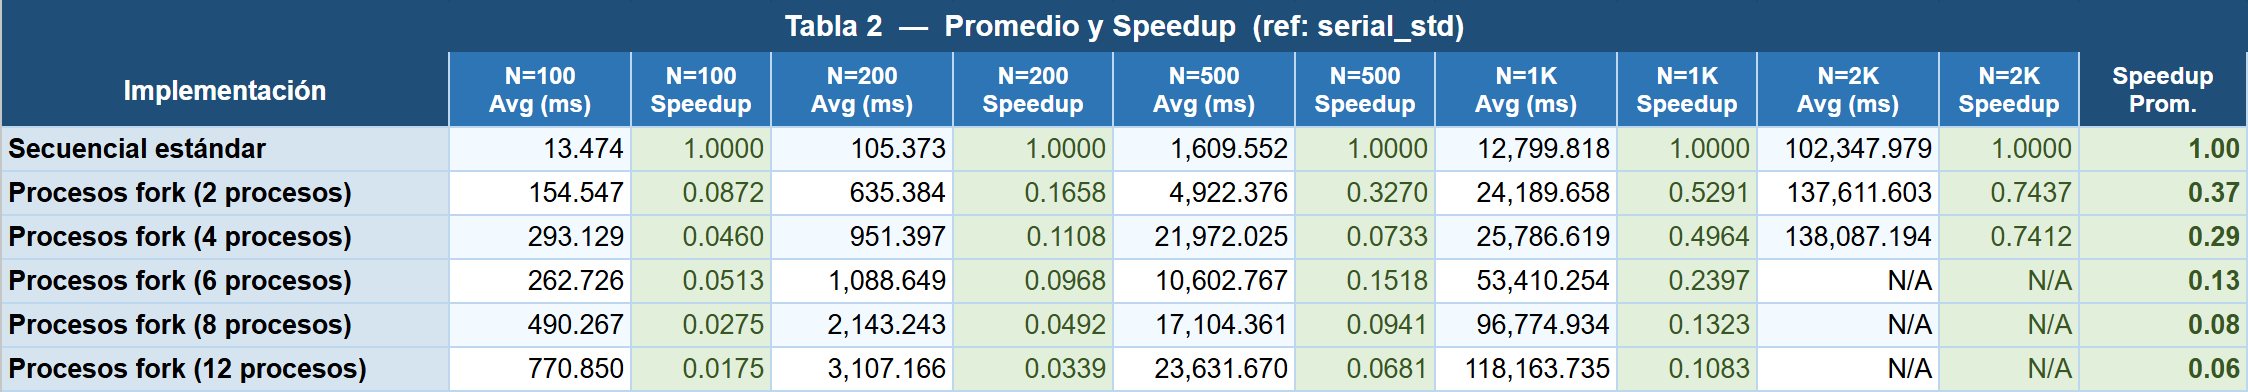
\includegraphics[width=1\textwidth]{images/tables/processes_speedup.png}
   \caption{Speedup del algoritmo paralelizado por procesos}
   \label{tab:processes_speedup}
\end{table}

\begin{figure}
   \centering
   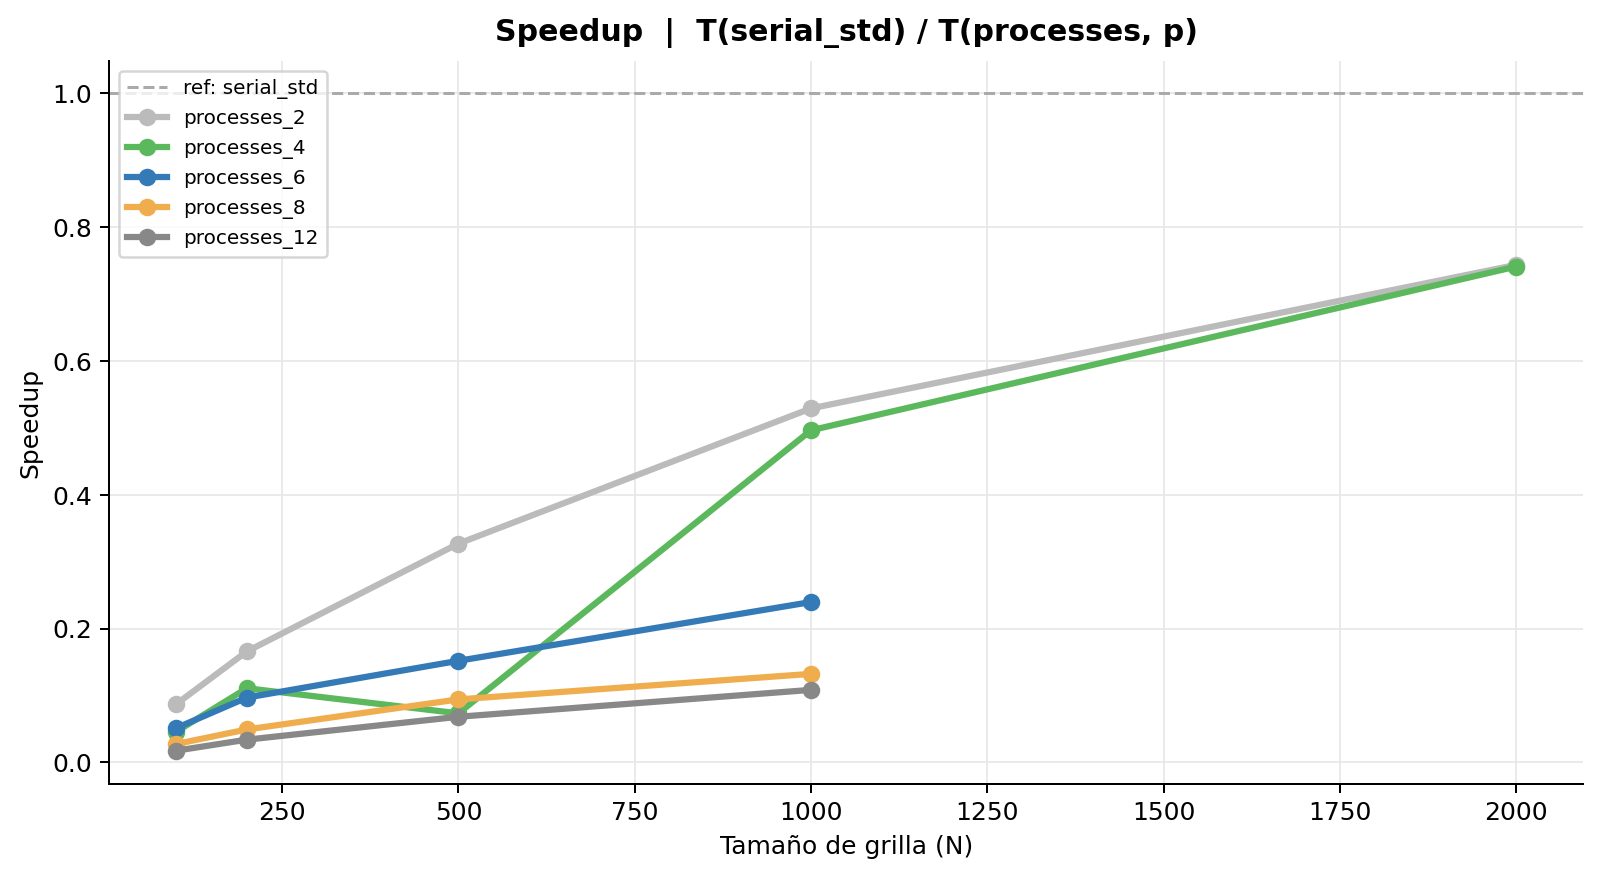
\includegraphics[width=1\textwidth]{images/charts/processes_sp.png}
   \caption{Comparación del speedup entre el algoritmo secuencial y el algoritmo paralelizado por procesos}
   \label{fig:chart_processes_speedup}
\end{figure}